\documentclass[convert={density=600,size=672x480,outext=.png}]{standalone}
\usepackage{tikz}
\usetikzlibrary{calc, shapes, positioning, decorations.text, arrows.meta,
                trees,positioning,arrows,chains,shapes.geometric,automata,%
                decorations.pathreplacing,decorations.pathmorphing,shapes,%
                matrix,shapes.symbols,plotmarks,decorations.markings,shadows}
\usepackage{tikzscale}
\usepackage{pgfplots}

\definecolor{mybluetikz}{RGB}{86,180,233}
\definecolor{myredtikz}{RGB}{213,94,0}
\definecolor{mygreen}{RGB}{124,174,0}

\definecolor[named]{myblue}{RGB}{0,102,204}
\definecolor[named]{myred}{RGB}{174,49,54}

\newcommand{\probinfevent}{\alpha}
\newcommand{\probbadnews}{\delta}

%%%%%%%%%%%%%%%%%%%%%%%%%%%%%%%%%%%%%%%%%%%%%%%%%
%
% Some definitions for TikZ graphics
%
%%%%%%%%%%%%%%%%%%%%%%%%%%%%%%%%%%%%%%%%%%%%%%%%%

\tikzset{
  root/.style = {rectangle,rounded corners, text width=7em, text centered, inner sep=2mm,
                 align = center, top color=white,
                 bottom color=blue!50!black!20, draw=blue!40!black!60, very thick},
  goodnode/.style = {rectangle, rounded corners, text width = 7em, text centered, inner sep = 2mm,
                     draw = mygreen!60,
                     top color = white, bottom color = mygreen!40, very thick},
  badnode/.style = {rectangle, rounded corners,text width = 7em, text centered, inner sep = 2mm,
                    draw = myredtikz!60,
                    top color = white, bottom color = myredtikz!40, very thick},
  nonode/.style = {rectangle, rounded corners, text width = 7em, text centered, inner sep = 2mm,
                   draw = mybluetikz!60,
                   top color = white, bottom color = mybluetikz!40, very thick}
}

\pgfplotsset{compat = 1.12,
     cmhplot/.style={color=mybluetikz,mark=none,line width=3pt,-},
     cmhplotouter/.style={color=mybluetikz!70,mark=none,line width=3pt,-},
     cmhplotobs/.style={color=mybluetikz,mark=none,line width=2pt,-},
     cmhplotbuys/.style={color=mygreen!40,mark=none,line width=1.5pt,-},
     cmhplotsells/.style={color=myredtikz!40,mark=none,line width=1.5pt,-},
     soldot/.style={color=myredtikz,only marks,mark=*, mark size = 3.5},
     holdot/.style={color=myredtikz,fill=white,only marks,mark=*, mark size = 3.5},
     soldotouter/.style={color=myredtikz!70,only marks,mark=*, mark size = 3.5},
     holdotouter/.style={color=myredtikz!70,fill=white,only marks,mark=*, mark size = 3.5},
     soldotbuys/.style={color=mygreen!40,only marks,mark=*, mark size = 2},
     holdotbuys/.style={color=mygreen!40,fill=white,only marks,mark=*, mark size = 2},
     holdotbuysreset/.style={color=mygreen!40,fill=white,only marks,mark=square*, mark size = 3},
     soldotsells/.style={color=myredtikz!40,only marks,mark=*, mark size = 2},
     holdotsells/.style={color=myredtikz!40,fill=white,only marks,mark=*, mark size = 2},
     holdotsellsreset/.style={color=myredtikz!40,fill=white,only marks,mark=square*, mark size = 3},
     soldotobs/.style={color=mybluetikz,only marks,mark=*, mark size = 2.5},
     holdotobs/.style={color=mybluetikz,fill=white,only marks,mark=*, mark size = 2.5},
}
\begin{document}
\tikzset{
  root/.style = {rectangle,rounded corners, text width=7em, text centered, inner sep=2mm,
                 align = center, top color=white,
                 bottom color=blue!50!black!20, draw=blue!40!black!60, very thick},
  goodnode/.style = {rectangle, rounded corners, text width = 7em, text centered, inner sep = 2mm,
                     draw = mygreen!60,
                     top color = white, bottom color = mygreen!40, very thick},
  badnode/.style = {rectangle, rounded corners,text width = 7em, text centered, inner sep = 2mm,
                    draw = myredtikz!60,
                    top color = white, bottom color = myredtikz!40, very thick},
  nonode/.style = {rectangle, rounded corners, text width = 7em, text centered, inner sep = 2mm,
                   draw = mybluetikz!60,
                   top color = white, bottom color = mybluetikz!40, very thick}
}

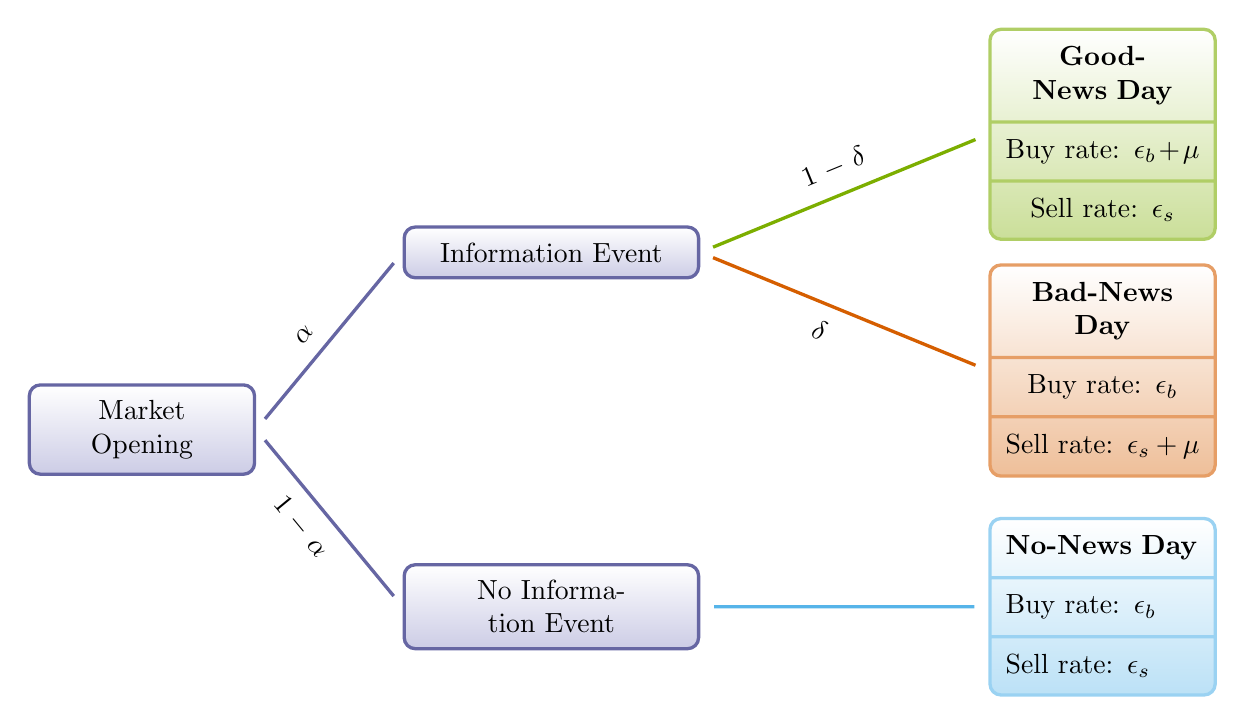
\begin{tikzpicture}[
    grow=right,
    level 1/.style={sibling distance=4.5cm,level distance=5.2cm},
    level 2/.style={sibling distance=3cm, level distance=7cm},
    edge from parent/.style={very thick,draw=blue!40!black!60,
                             shorten >=5pt, shorten <=5pt},
    edge from parent path={(\tikzparentnode.east) -- (\tikzchildnode.west)},
    kant/.style={text width=2cm, text centered, sloped},
    every node/.style={text ragged, inner sep=2mm},
    punkt/.style={rectangle, rounded corners, shade, top color=white, align = center,
                  bottom color=blue!50!black!20, draw=blue!40!black!60, very thick }
    ]

\node[punkt, text width=7em] {Market Opening}
    child{ %Lower part lv1
        node[punkt, text width=9.5em] {No Information Event}
        child {
            node[nonode] [rectangle split, rectangle split, rectangle split parts=3,
             text ragged] {
                \textbf{No-News Day}
                      \nodepart{second}
                Buy rate: $\epsilon_b$
                      \nodepart{third}
                Sell rate: $\epsilon_s$
            }
            edge from parent [draw = mybluetikz]
                node[kant, below, pos=.45] {}}
        edge from parent
                node[kant, below, pos = 0.45] {$1 - \probinfevent$}
    }
    %Upper part, lv1
    child {
        node[punkt, text width=9.5em] {Information Event}
        %child 1
        child {
            node [badnode,rectangle split, rectangle split,
            rectangle split parts=3] {
                \textbf{Bad-News Day}
                \nodepart{second}
                Buy rate: $\epsilon_b$
                \nodepart{third}
                Sell rate: $\epsilon_s + \mu$
            }
            edge from parent [draw = myredtikz]
                node[below, kant,  pos=.45] {$\probbadnews$}}
        % }
        %child 2
        child {
            node [goodnode, rectangle split, rectangle split parts=3]{
                \textbf{Good-News Day}
                \nodepart{second}
                Buy rate: $\epsilon_b + \mu$
                \nodepart{third}
                Sell rate: $\epsilon_s$
            }
            edge from parent [draw = mygreen]
                node[kant, above] {$1 - \probbadnews$}}
            edge from parent
                node[kant, above, pos = 0.45] {$\probinfevent$}
    };
\end{tikzpicture}
\end{document}